
%人类对这种能力的应用,大致可以分为两类:有意识的和无意识的。在有意识的情况下,人类在视觉场景中主动寻找目标物体,并对其定位,这通常是任务驱动的(比如在餐厅中寻找自己的同伴);在无意识的情况下,人类被动的接受视觉场景,并对场景中的某些部分产生无意识的视觉停留(比如颜色鲜艳的物体通常更容易吸引人类的注意力)。

\chapter{绪论}
对于人类而言,在一个视觉场景中迅速找到并定位自己所感兴趣的物体,是非常自然且简单的事情。然而对于计算机而言,目标的检测与识别却是一项十分艰难的任务。更为重要的是,许多计算机视觉中的问题,都将物体的检测与定位作为一个必不可缺的预处理步骤,目标检测的精度将直接影响到后续的处理效果。然而到目前为止,许多经典的物体检测与定位方法都是类别相关的,也就是说,这些方法大多只能检测或定位特定类别的物体(比如人脸,车辆、行人等等)。 近年来逐渐流行起来的显著性区域检测方法,为类别无关的物体检测与定位提供了一个思路。本章主要介绍了显著性区域检测的一些基本概念与历史,并对国内外的研究现状进行了简要的概括。

\section{课题研究的背景与意义}
图像作为记录信息、传递思想和表达情感的重要媒介,在现代人的日常生活中扮演了重要角色。另外随着智能手机和数码相机等硬件设备的普及,人们创造、获取图像的手段也日益方便与灵活。再加上近年来社交网络、微博、网络相册等共享平台快速兴起,以及图像本身所具有的内容直观、获取容易、传播方便、表现力丰富等优势,数字图像迅速成为日常生活中最受欢迎的一种知识传播和信息共享媒介\cite{CMM12THU}。对互联网上海量的数字图像进行处理与应用,挖掘出人们所需的信息,不仅会给人们带来许多便利,同时也蕴含了极大的商业价值。

\begin{figure}[h]
\centering
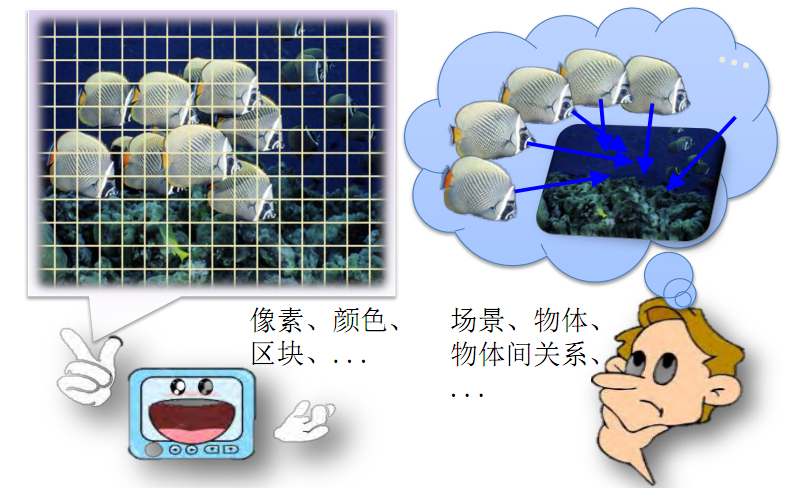
\includegraphics[width=0.8\textwidth]{relationship.jpg}
\caption{计算机与人类对图像处理的差异}
\end{figure}

然而,计算机对图像的处理方式与人类有着极大的不同。计算机以像素为基本单位,通过记录像素的颜色以及像素间的排列关系来存储、处理图像,这是一种非常低阶的处理手段;而人类则是通过高阶概念,如场景、物体、及物体间相互关系为基本处理单位,对图像进行认知和记忆。这种本质上的差异,导致目前计算机对图像的理解与处理远远不能与人类相比。因此,从某种程度上来讲,要想有效减小计算机与人类在图像处理方面的差距,必须首先解决计算机从离散的像素到更高层次的认知单位的映射问题。譬如传统的图像分割,则是希望将一群离散的像素映射组织为若干有共同属性、含义的基本语义单元。

更为重要的是,在当前大数据时代的背景下,对海量图像进行快速有效的处理更加成为了一个亟待解决的问题。然而,正如前面所讲到的,如果继续以像素为基本处理单位,很难实时有效的处理这些图像数据。假如我们能够将图像中人类感兴趣的区域提取出来,不仅减小了后续处理的工作量,同时也从语义级别对像素进行了一次映射,这将是大有裨益的。

\begin{figure}[b]
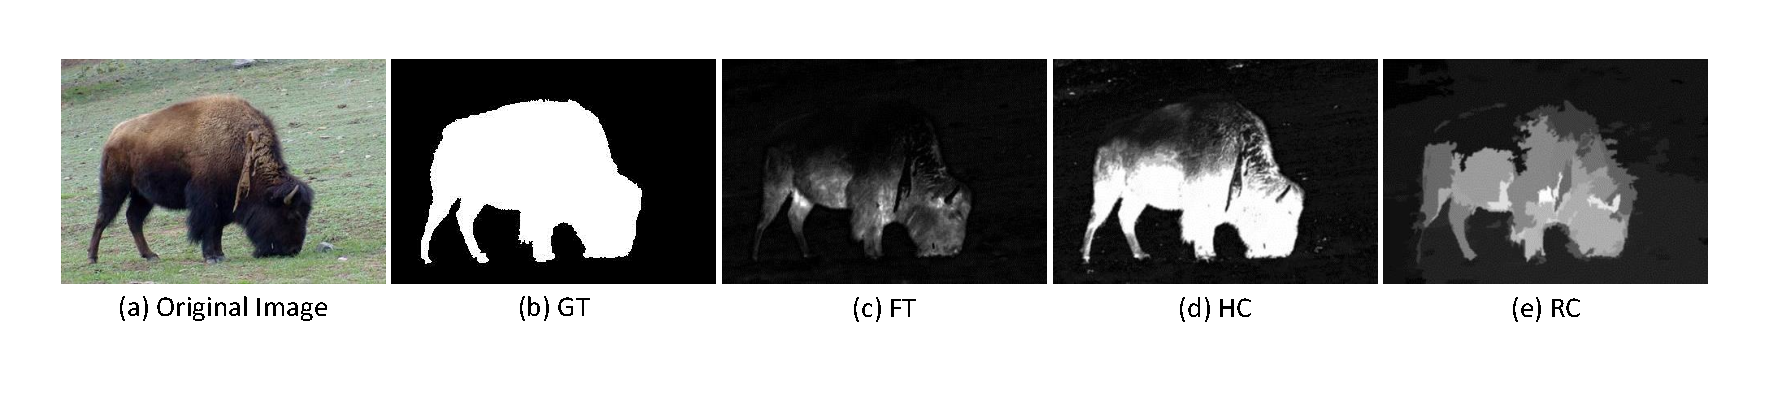
\includegraphics[width=\textwidth]{intro.pdf}
\caption{显著性区域检测示例}\label{fig:intro}
\end{figure}

在这样的需求推动下,显著性区域检测成为了一个研究热点。所谓显著性区域,即一幅图像中最能吸引人类注意力的区域,通常为一幅图像的前景物体。而显著性区域检测的目标,即通过一个与原图像大小相同的二值图像,来标明哪些区域是显著的。如图\ref{fig:intro}所示,(a)是源图像,(b)为一个二值标准图像(Ground Truth),用来标示哪些像素点是显著的。当然,一般的显著性区域检测方法不可能做到精确的标示哪些像素显著与否。因此,显著性区域检测的方法大多产生一个灰度图像,其中灰度值越高,表明这个像素的显著程度越高,如图\ref{fig:intro}.(c)(d)(e)所示,分别为FT\cite{achanta2009frequency},HC\cite{cheng2011global},RC\cite{cheng2011global}三种方法所产生的显著图。

作为一种通用物体的定位与检测手段,显著区域检测可以很好的与其他应用相结合以提升效果,比如图像检索\cite{tsai2012hierarchical}\cite{fang2012effective},图像的自动裁剪\cite{shechtman2013methods}\cite{deigmoeller2010context},自适应图像压缩\cite{christopoulos2000jpeg2000},以及图像分割\cite{jiang2011automatic}\cite{han2006unsupervised},等等。正是由于其广泛的应用,显著区域检测得到了来自许多不同领域学者的关注,对显著性区域的准确快速的定位,将会对计算机视觉、多媒体内容分析等领域产生十分积极的影响。

\section{国内外研究现状}
对于人类视觉注意力的研究,可以追溯到Koch和Ullman\cite{koch1987shifts}的基于生物视觉特性的计算模型。随后,显著区域检测的开创者Itti\cite{itti1998model}在此模型的基础上进行了改进,通过结合多尺度的图像特征,在快速场景识别上取得了很好的效果。自此以后,显著区域检测就吸引了大批学者的注意。

在最初的阶段,人们受到生物视觉特性的启发,即与周围环境差异较大,有较强对比度的区域通常更能引起人们的注意,因此人们大多采用基于局部对比度的方法。在Ma和Zhang的工作中\cite{ma2003contrast},基于局部对比度的分析方法被首次正式提出,通过进一步结合模糊集理论(Fuzzy Theory),就可以得到一幅图像的显著区域。在Harel等人的工作中\cite{harel2006graph},根据像素点之间的相似性,首先构建了一个图(Graph),随后通过马尔科夫过程的收敛性,挖掘图像区域的独特性,并对差异较大、较为独特的区域赋予较大的显著值。其他的一些学者,比如Liu\cite{liu2011learning}和Mai\cite{maisaliency}等人,同样也将局部对比度作为一个重要的特征来发掘显著性区域。然而,基于局部对比度的方法有一个很大的缺陷,他们倾向于给物体边缘赋予较大的显著值,而并非高亮整个显著区域。

最近的几年,基于全局对比度的方法越来越流行,他们能够高亮整个区域,而并非边缘。Zhai等人\cite{zhai2006visual}提出了第一个基于全局对比度的模型,一个像素的显著性被定义为与图像中所有其他像素的差异度之和。考虑到计算性能问题,他们仅仅采用了像素的亮度信息来度量像素之间的差异,而忽略了颜色信息。Cheng等人\cite{cheng2011global}注意到了这一点,充分利用了一个像素的三个颜色通道来度量像素差异。为了使计算足够高效同时又保持良好的效果,他们提出了两个解决方法,即基于颜色直方图的加速和色彩空间平滑。在Cheng等人的工作发表后,学者们注意到了基于全局对比度方法的良好效果与计算可行性,自此以后,大多最近的工作都将全局对比度作为重要的特征用来提取显著区域。

除了上述基于对比度的模型(即挖掘像素点或区域的独特性),还有另外一些基于频域分析的模型\cite{achanta2009frequency}\cite{hou2007saliency}\cite{hou2012image},这些模型通过将图像映射到频域进行分析,并结合信号处理与数据压缩理论,能提取出一幅图像中的独特部分,有着良好的理论支持。然而,\cite{hou2012image}指出,这些基于频域分析的模型在某种程度上等同于一个局部梯度算子并叠加一个高斯模糊,因此在检测较大的显著区域时表现较差。

另外,近年来随着机器学习的流行,也有一些学者尝试基于学习的模型。Kienzel等人\cite{kienzle2007nonparametric}利用支持向量机(SVM)从已有的眼动数据学习得到了一个显著区域检测模型。Mai等人\cite{maisaliency}使用条件随机场(CRF)结合多个显著图,并充分利用了相邻像素之间的关联性来建立模型。尽管这些基于学习的方法在现有的数据集下能取得不错的效果,但是他们通常都十分耗时,同时由于机器学习对于学习数据的强依赖性,导致这类方法在不同数据集下的表现也存在较大的差异。

可以看到,国际上对于显著性区域检测的研究正呈现百花齐放的状态,各个学者对显著性区域检测都有不同的理解与思考,同时也产生了完全不同的算法与思路,这也恰好说明了人们对于显著性区域检测这一课题还处于初级探索阶段,还未形成统一的见解与共识。

\section{本文所做的工作}
作为一种通用的物体检测手段,显著性区域有着极其广阔的应用空间\cite{tsai2012hierarchical}\cite{fang2012effective}\cite{deigmoeller2010context}\cite{jiang2011automatic}。在如此巨大的需求推动下,本文围绕显著性区域检测的算法以及相关应用进行了研究,主要工作与成果如下:

\begin{enumerate}
\item 通过对不同特征的分析,提出了基于多特征结合的显著性区域检测算法。该算法首先提出了四个基本的显著性区域特征,随后通过条件随机场(CRF)建模,学习多个特征在多个尺度下的相互关联与互补关系。算法能够有效的检测图像中的视觉显著区域,并且在目前国际标准数据集上取得了良好的效果。为了验证该算法的性能,在两个国际标准数据集上,我们对比了国际上现有的十余种经典算法,实验结果显示,我们的算法具有很高的精确率与召回率,同时还有相对鲁棒的特性。
\item 通过观察空间约束对显著性区域检测的影响,我们提出了基于蒙特卡洛采样的显著性区域检测算法。该算法提出了三种有效的空间约束关系:紧致性、连通性、包络性。为了有效的利用这三种空间约束关系,我们创造性的提出了利用蒙特卡洛采样,将空间约束加入现有特征中的方法。同时,这一方案有着非常高的时间效率,而采样的高度可并行化,使得实时计算显著性区域成为可能,大大提高了算法的实用价值。
\item 显著性区域检测的真正价值在于它的应用,我们尝试将显著性区域检测应用在人脸识别和图像检索中,并探讨了一些可行性方案,最后通过实验论证了显著性区域检测所带来的优化效果。
\end{enumerate}

\section{论文组织结构}
本文分为五章,主要结构和内容如下:

第一章首先阐述了显著性区域检测的研究背景和意义,接着介绍了该方向的国内外研究现状以及存在的问题,最后概述了本文所做的工作和论文的组织结构。

第二章介绍了显著性区域检测的基础特征与算法,并分类探讨了目前国际上各类主流算法的思路与不足。在这一章的末尾,还介绍了该领域最新的研究进展与趋势。

第三章介绍本文提出的,基于条件随机场的多特征结合算法,并通过实验详细比较了该算法的优势与不足。

第四章介绍本文提出的,基于蒙特卡洛采样、结合空间约束特征的算法。

第五章探讨了显著性区域检测应用在人脸识别和图像检索上的价值,对存在的问题和局限性进行了讨论,最后对全文进行了总结,同时展望未来的研究工作。
